\subsection{Gtransfo\-Cub  Class Reference}
\label{class_gtransfocub}\index{GtransfoCub@{Gtransfo\-Cub}}
implements the cubic transformations (20 real coefficients). 


{\tt \#include $<$gtransfo.h$>$}

Inheritance diagram for Gtransfo\-Cub::\begin{figure}[H]
\begin{center}
\leavevmode
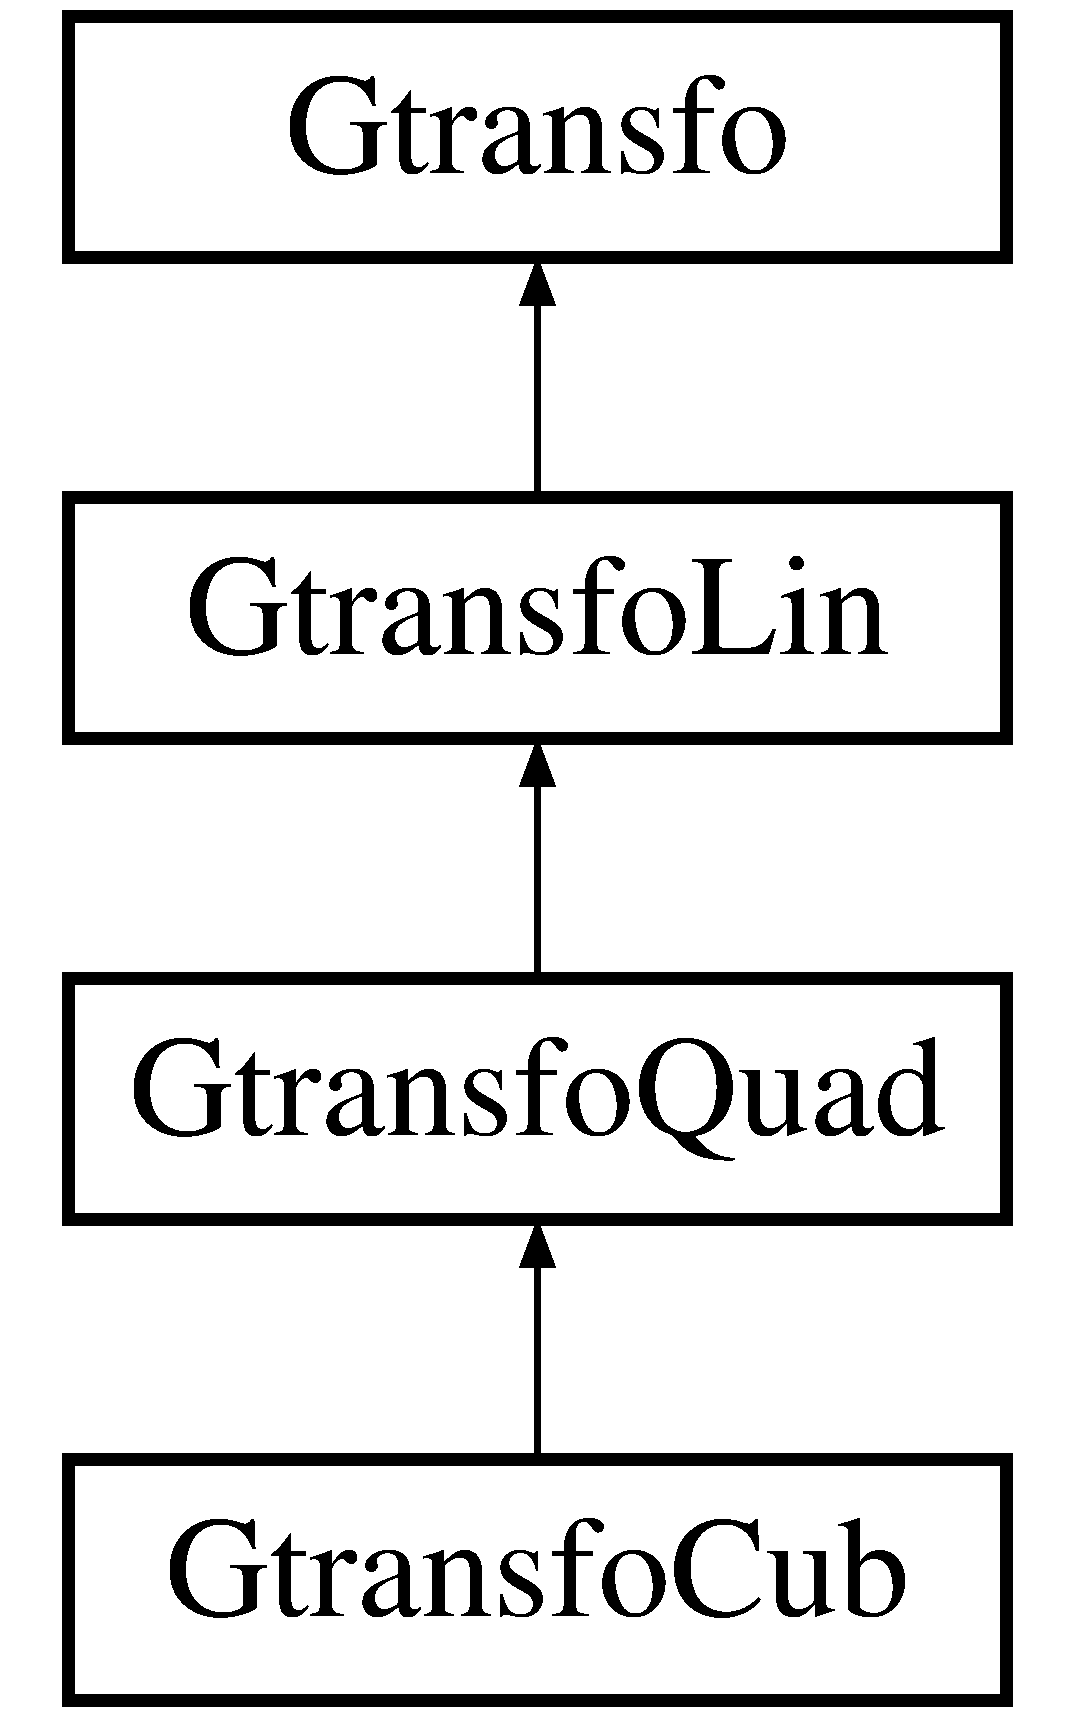
\includegraphics[height=4cm]{class_gtransfocub}
\end{center}
\end{figure}
\subsubsection*{Public Types}
\begin{CompactItemize}
\item 
enum {\bf Old\-Or\-New} \{ {\bf Old}, 
{\bf New}
 \}
\end{CompactItemize}
\subsubsection*{Public Methods}
\begin{CompactItemize}
\item 
\index{GtransfoCub@{GtransfoCub}!GtransfoCub@{Gtransfo\-Cub}}\index{GtransfoCub@{GtransfoCub}!GtransfoCub@{Gtransfo\-Cub}}
{\bf Gtransfo\-Cub} ()\label{class_gtransfocub_a0}

\begin{CompactList}\small\item\em the default constructor constructs the do-nothing transformation.\item\end{CompactList}\item 
\index{GtransfoCub@{GtransfoCub}!GtransfoCub@{Gtransfo\-Cub}}\index{GtransfoCub@{GtransfoCub}!GtransfoCub@{Gtransfo\-Cub}}
{\bf Gtransfo\-Cub} (const {\bf Gtransfo\-Lin} \&Lin)\label{class_gtransfocub_a1}

\begin{CompactList}\small\item\em upgrade a linear transfo to a cubic one.\item\end{CompactList}\item 
\index{GtransfoCub@{GtransfoCub}!GtransfoCub@{Gtransfo\-Cub}}\index{GtransfoCub@{GtransfoCub}!GtransfoCub@{Gtransfo\-Cub}}
{\bf Gtransfo\-Cub} (const {\bf Gtransfo\-Quad} \&Quad)\label{class_gtransfocub_a2}

\begin{CompactList}\small\item\em upgrade a quadratic transfo to a cubic one.\item\end{CompactList}\item 
\index{apply@{apply}!GtransfoCub@{Gtransfo\-Cub}}\index{GtransfoCub@{GtransfoCub}!apply@{apply}}
void {\bf apply} (const double Xin, const double Yin, double \&Xout, double \&Yout) const\label{class_gtransfocub_a3}

\item 
\index{apply@{apply}!GtransfoCub@{Gtransfo\-Cub}}\index{GtransfoCub@{GtransfoCub}!apply@{apply}}
{\bf Point} {\bf apply} (const {\bf Point} \&Pin)\label{class_gtransfocub_a4}

\item 
\index{dump@{dump}!GtransfoCub@{Gtransfo\-Cub}}\index{GtransfoCub@{GtransfoCub}!dump@{dump}}
void {\bf dump} (ostream \&stream=cout) const\label{class_gtransfocub_a5}

\begin{CompactList}\small\item\em dumps the transfo coefficients to stream.\item\end{CompactList}\item 
double {\bf fit} (const Star\-Match\-List \&List, const {\bf Gtransfo} $\ast$Prior\-Transfo=NULL, const {\bf Gtransfo} $\ast$Posterior\-Transfo=NULL)
\item 
\index{Clone@{Clone}!GtransfoCub@{Gtransfo\-Cub}}\index{GtransfoCub@{GtransfoCub}!Clone@{Clone}}
{\bf Gtransfo}$\ast$ {\bf Clone} () const\label{class_gtransfocub_a7}

\begin{CompactList}\small\item\em returns a copy (allocated by new) of the transformation.\item\end{CompactList}\item 
\index{ReduceCompo@{ReduceCompo}!GtransfoCub@{Gtransfo\-Cub}}\index{GtransfoCub@{GtransfoCub}!ReduceCompo@{Reduce\-Compo}}
{\bf Gtransfo}$\ast$ {\bf Reduce\-Compo} (const {\bf Gtransfo} $\ast$Right) const\label{class_gtransfocub_a8}

\begin{CompactList}\small\item\em allow composition of transformations regardless of their actual types.see {\bf Gtransfo\-Compose}() {\rm (p.\,\pageref{gtransfo_h_a1})} for a user callable entry.\item\end{CompactList}\item 
\index{dX@{dX}!GtransfoCub@{Gtransfo\-Cub}}\index{GtransfoCub@{GtransfoCub}!dX@{d\-X}}
double {\bf d\-X} () const\label{class_gtransfocub_a9}

\item 
\index{dY@{dY}!GtransfoCub@{Gtransfo\-Cub}}\index{GtransfoCub@{GtransfoCub}!dY@{d\-Y}}
double {\bf d\-Y} () const\label{class_gtransfocub_a10}

\item 
\index{A11@{A11}!GtransfoCub@{Gtransfo\-Cub}}\index{GtransfoCub@{GtransfoCub}!A11@{A11}}
double {\bf A11} () const\label{class_gtransfocub_a11}

\item 
\index{A12@{A12}!GtransfoCub@{Gtransfo\-Cub}}\index{GtransfoCub@{GtransfoCub}!A12@{A12}}
double {\bf A12} () const\label{class_gtransfocub_a12}

\item 
\index{A21@{A21}!GtransfoCub@{Gtransfo\-Cub}}\index{GtransfoCub@{GtransfoCub}!A21@{A21}}
double {\bf A21} () const\label{class_gtransfocub_a13}

\item 
\index{A22@{A22}!GtransfoCub@{Gtransfo\-Cub}}\index{GtransfoCub@{GtransfoCub}!A22@{A22}}
double {\bf A22} () const\label{class_gtransfocub_a14}

\item 
\index{A1X2@{A1X2}!GtransfoCub@{Gtransfo\-Cub}}\index{GtransfoCub@{GtransfoCub}!A1X2@{A1X2}}
double {\bf A1X2} () const\label{class_gtransfocub_a15}

\item 
\index{A1XY@{A1XY}!GtransfoCub@{Gtransfo\-Cub}}\index{GtransfoCub@{GtransfoCub}!A1XY@{A1XY}}
double {\bf A1XY} () const\label{class_gtransfocub_a16}

\item 
\index{A1Y2@{A1Y2}!GtransfoCub@{Gtransfo\-Cub}}\index{GtransfoCub@{GtransfoCub}!A1Y2@{A1Y2}}
double {\bf A1Y2} () const\label{class_gtransfocub_a17}

\item 
\index{A2X2@{A2X2}!GtransfoCub@{Gtransfo\-Cub}}\index{GtransfoCub@{GtransfoCub}!A2X2@{A2X2}}
double {\bf A2X2} () const\label{class_gtransfocub_a18}

\item 
\index{A2XY@{A2XY}!GtransfoCub@{Gtransfo\-Cub}}\index{GtransfoCub@{GtransfoCub}!A2XY@{A2XY}}
double {\bf A2XY} () const\label{class_gtransfocub_a19}

\item 
\index{A2Y2@{A2Y2}!GtransfoCub@{Gtransfo\-Cub}}\index{GtransfoCub@{GtransfoCub}!A2Y2@{A2Y2}}
double {\bf A2Y2} () const\label{class_gtransfocub_a20}

\item 
\index{A1X3@{A1X3}!GtransfoCub@{Gtransfo\-Cub}}\index{GtransfoCub@{GtransfoCub}!A1X3@{A1X3}}
double {\bf A1X3} () const\label{class_gtransfocub_a21}

\item 
\index{A1X2Y@{A1X2Y}!GtransfoCub@{Gtransfo\-Cub}}\index{GtransfoCub@{GtransfoCub}!A1X2Y@{A1X2Y}}
double {\bf A1X2Y} () const\label{class_gtransfocub_a22}

\item 
\index{A1XY2@{A1XY2}!GtransfoCub@{Gtransfo\-Cub}}\index{GtransfoCub@{GtransfoCub}!A1XY2@{A1XY2}}
double {\bf A1XY2} () const\label{class_gtransfocub_a23}

\item 
\index{A1Y3@{A1Y3}!GtransfoCub@{Gtransfo\-Cub}}\index{GtransfoCub@{GtransfoCub}!A1Y3@{A1Y3}}
double {\bf A1Y3} () const\label{class_gtransfocub_a24}

\item 
\index{A2X3@{A2X3}!GtransfoCub@{Gtransfo\-Cub}}\index{GtransfoCub@{GtransfoCub}!A2X3@{A2X3}}
double {\bf A2X3} () const\label{class_gtransfocub_a25}

\item 
\index{A2X2Y@{A2X2Y}!GtransfoCub@{Gtransfo\-Cub}}\index{GtransfoCub@{GtransfoCub}!A2X2Y@{A2X2Y}}
double {\bf A2X2Y} () const\label{class_gtransfocub_a26}

\item 
\index{A2XY2@{A2XY2}!GtransfoCub@{Gtransfo\-Cub}}\index{GtransfoCub@{GtransfoCub}!A2XY2@{A2XY2}}
double {\bf A2XY2} () const\label{class_gtransfocub_a27}

\item 
\index{A2Y3@{A2Y3}!GtransfoCub@{Gtransfo\-Cub}}\index{GtransfoCub@{GtransfoCub}!A2Y3@{A2Y3}}
double {\bf A2Y3} () const\label{class_gtransfocub_a28}

\item 
\index{GetValues@{GetValues}!GtransfoCub@{Gtransfo\-Cub}}\index{GtransfoCub@{GtransfoCub}!GetValues@{Get\-Values}}
void {\bf Get\-Values} (vector$<$ {\bf Named\-Value} $>$ \&Values, const Old\-Or\-New Which\-Names=New) const\label{class_gtransfocub_a29}

\item 
\index{SetValues@{SetValues}!GtransfoCub@{Gtransfo\-Cub}}\index{GtransfoCub@{GtransfoCub}!SetValues@{Set\-Values}}
void {\bf Set\-Values} (vector$<$ {\bf Named\-Value} $>$ \&Values)\label{class_gtransfocub_a30}

\item 
\index{Npar@{Npar}!GtransfoCub@{Gtransfo\-Cub}}\index{GtransfoCub@{GtransfoCub}!Npar@{Npar}}
int {\bf Npar} () const\label{class_gtransfocub_a31}

\begin{CompactList}\small\item\em returns the number of parameters (to compute chi2's).\item\end{CompactList}\item 
\index{Degree@{Degree}!GtransfoCub@{Gtransfo\-Cub}}\index{GtransfoCub@{GtransfoCub}!Degree@{Degree}}
virtual int {\bf Degree} () const\label{class_gtransfocub_a32}

\end{CompactItemize}
\subsubsection*{Protected Methods}
\begin{CompactItemize}
\item 
\index{identity@{identity}!GtransfoCub@{Gtransfo\-Cub}}\index{GtransfoCub@{GtransfoCub}!identity@{identity}}
void {\bf identity} ()\label{class_gtransfocub_b0}

\end{CompactItemize}
\subsubsection*{Protected Attributes}
\begin{CompactItemize}
\item 
\index{a1x3@{a1x3}!GtransfoCub@{Gtransfo\-Cub}}\index{GtransfoCub@{GtransfoCub}!a1x3@{a1x3}}
double {\bf a1x3}\label{class_gtransfocub_n0}

\item 
\index{a1x2y@{a1x2y}!GtransfoCub@{Gtransfo\-Cub}}\index{GtransfoCub@{GtransfoCub}!a1x2y@{a1x2y}}
double {\bf a1x2y}\label{class_gtransfocub_n1}

\item 
\index{a1xy2@{a1xy2}!GtransfoCub@{Gtransfo\-Cub}}\index{GtransfoCub@{GtransfoCub}!a1xy2@{a1xy2}}
double {\bf a1xy2}\label{class_gtransfocub_n2}

\item 
\index{a1y3@{a1y3}!GtransfoCub@{Gtransfo\-Cub}}\index{GtransfoCub@{GtransfoCub}!a1y3@{a1y3}}
double {\bf a1y3}\label{class_gtransfocub_n3}

\item 
\index{a2x3@{a2x3}!GtransfoCub@{Gtransfo\-Cub}}\index{GtransfoCub@{GtransfoCub}!a2x3@{a2x3}}
double {\bf a2x3}\label{class_gtransfocub_n4}

\item 
\index{a2x2y@{a2x2y}!GtransfoCub@{Gtransfo\-Cub}}\index{GtransfoCub@{GtransfoCub}!a2x2y@{a2x2y}}
double {\bf a2x2y}\label{class_gtransfocub_n5}

\item 
\index{a2xy2@{a2xy2}!GtransfoCub@{Gtransfo\-Cub}}\index{GtransfoCub@{GtransfoCub}!a2xy2@{a2xy2}}
double {\bf a2xy2}\label{class_gtransfocub_n6}

\item 
\index{a2y3@{a2y3}!GtransfoCub@{Gtransfo\-Cub}}\index{GtransfoCub@{GtransfoCub}!a2y3@{a2y3}}
double {\bf a2y3}\label{class_gtransfocub_n7}

\end{CompactItemize}
\subsubsection*{Friends}
\begin{CompactItemize}
\item 
\index{operator *@{operator $\ast$}!GtransfoCub@{Gtransfo\-Cub}}\index{GtransfoCub@{GtransfoCub}!operator *@{operator $\ast$}}
Gtransfo\-Cub {\bf operator $\ast$} (const Gtransfo\-Cub \&L, const {\bf Gtransfo\-Lin} \&R)\label{class_gtransfocub_l0}

\begin{CompactList}\small\item\em Cub$\ast$Lin.\item\end{CompactList}\item 
\index{operator *@{operator $\ast$}!GtransfoCub@{Gtransfo\-Cub}}\index{GtransfoCub@{GtransfoCub}!operator *@{operator $\ast$}}
Gtransfo\-Cub {\bf operator $\ast$} (const {\bf Gtransfo\-Lin} \&L, const Gtransfo\-Cub \&R)\label{class_gtransfocub_l1}

\begin{CompactList}\small\item\em Lin$\ast$Cub.\item\end{CompactList}\end{CompactItemize}


\subsubsection{Detailed Description}
implements the cubic transformations (20 real coefficients).



\subsubsection{Member Function Documentation}
\index{GtransfoCub@{Gtransfo\-Cub}!fit@{fit}}
\index{fit@{fit}!GtransfoCub@{Gtransfo\-Cub}}
\paragraph{\setlength{\rightskip}{0pt plus 5cm}double Gtransfo\-Cub::fit (const Star\-Match\-List \& {\em List}, const {\bf Gtransfo} $\ast$ {\em Prior\-Transfo} = NULL, const {\bf Gtransfo} $\ast$ {\em Posterior\-Transfo} = NULL)\hspace{0.3cm}{\tt  [virtual]}}\hfill\label{class_gtransfocub_a6}


fits a transfo to a list of star pairs (p1,p2). After the fit this(Prior\-Transfo(p1)) yields approximately p2. The returned value is the chi2. 

Reimplemented from {\bf Gtransfo\-Quad} {\rm (p.\,\pageref{class_gtransfoquad_a5})}.

The documentation for this class was generated from the following file:\begin{CompactItemize}
\item 
{\bf gtransfo.h}\end{CompactItemize}
